\section{Design}
\label{sec:design}

Two main elements were needed in Beerculator's interface : one to get the user information (weight, gender, etc) and one to display its list of drinks. Also, a button was required for the user to indicate when to launch the calculation. The user interface can be seen on {\sc figure}~\ref{fig:ui}\\

On the left part of the interface, the user can add all informations that Beerculator needs from him. He can indicate its gender (male or female) via two check boxes, and its weight thanks to a text box. Another text box is also available for him to tell the number of hours since his drinking began. Finally, the user can select his drinks among the list of drinks predefined in the database. \\

Those drinks then appear in a list on the right side of the web page, which is dynamically updated as long as the user adds drinks. When he is done, the user can then click on the \guillemotleft Calculate \guillemotright button so that Beerculator starts the computation. The results appear in text blocks, under the list of drinks. First the BAC value is indicated, and under it the number of hours before the user gets sober again.\\

\begin{figure}[H]
\centering
   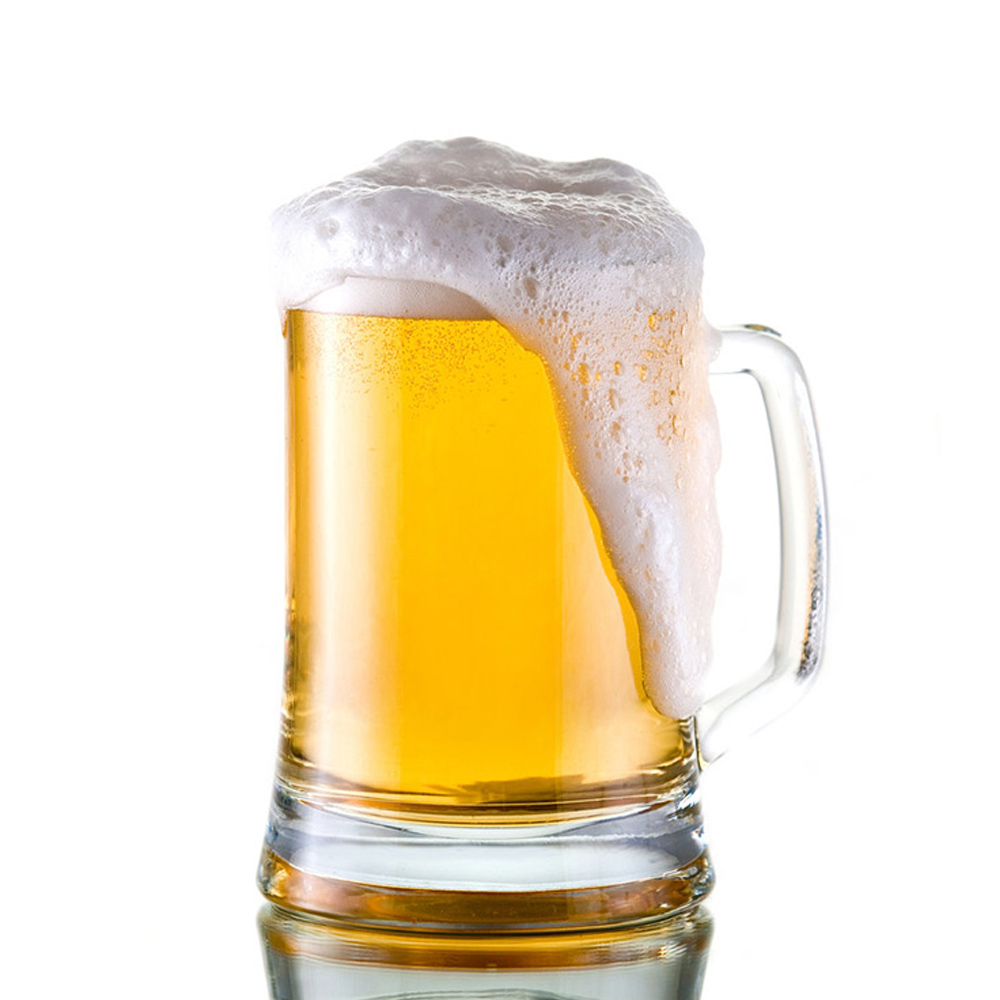
\includegraphics[scale=0.3]{./figures/beer.jpg}
   \caption{User interface of Beerculator}
   \label{fig:ui}
\end{figure}